\graphicspath{ {./images/8_Site_occupancy} }
\newpage

\section{Site occupancy (optional)}
GlycoDash will automatically detect the presence of non-glycosylated peptides in your data.
These are ignored during spectral and analyte curation. 
When a non-glycosylated peptide is present for a glycosylation site, this peptide can be used to calculate the corresponding site occupancy (e.g., when there are analytes \textsf{IgGI1H3N4F1}, \textsf{IgGI1H4N4F1}, etc. in your data, the analyte \textsf{IgGI1} without a glycan composition can be used).

\begin{wrapfigure}{R}{0.47\textwidth}
	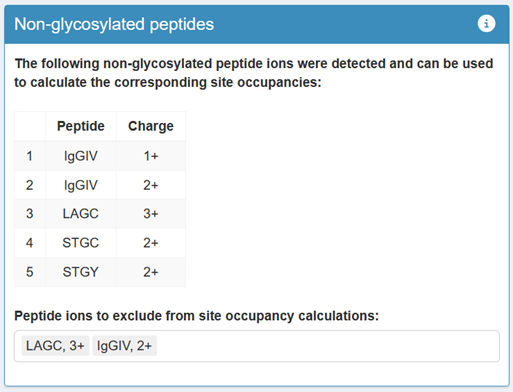
\includegraphics[scale=0.55]{peptides_table.png}
\end{wrapfigure}

The detected non-glycosylated peptides and their charge states are listed in a table, and corresponding site occupancies are automatically calculated.
You have the option to exclude ions from the site occupancy calculations, such as when the quality is insufficient (see below).
When you exclude all charge states for a peptide, the corresponding site occupancy is not calculated.

In the \textsf{Quality check} box, the quality of each detected peptide ion is visualized.
The percentage of samples in which the ion fulfills three quality criteria is plotted, with the option to exclude certain sample types from the assessment.
For $S/N$ and IPQ (SweetSuite and LaCyTools data), or total area and IDP (Skyline data), the same criteria that were used for spectral and analyte curation are applied.
Because non-glycosylated peptides are often quantified without internal calibration, you may want to be more lenient when it comes to the acceptable mass error. 
This value can therefore be set manually here.

\begin{center}
	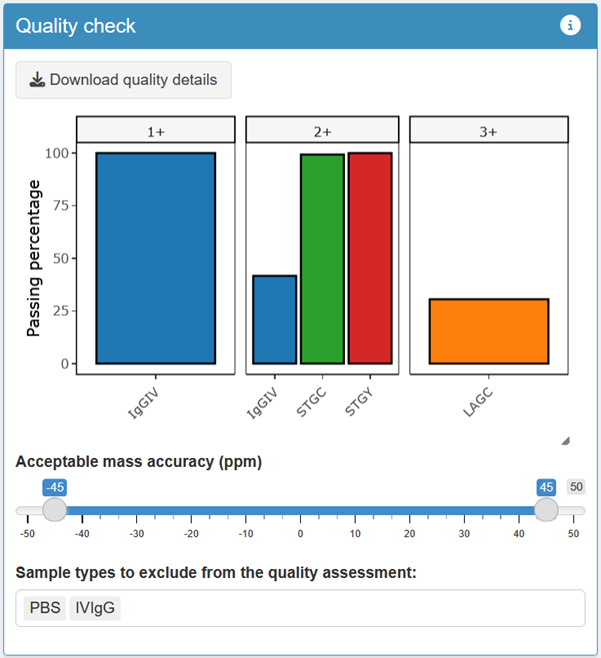
\includegraphics[scale=0.6]{peptides_quality.png}
\end{center}